\chapter{Goby MOOS Modules}\label{chap:MOOS}
\MakeShortVerb{\!} % makes !foo! == !foo!

The acoustic communications portion of Goby was developed originally for the MOOS autonomy architecture. Thus, the relevant MOOS modules !pAcommsHandler! and others are still maintained (in goby/src/moos) for the use of the !MOOS-IvP! community. !MOOS-IvP! is explained in \cite{moos-ivp-jfr} and is available at \url{http://moos-ivp.org}. The usage of these modules is documented here. See \url{http://gobysoft.org/wiki/InstallingGoby} for how to install Goby.


\section{Goby MOOS Applications} \label{sec:goby_moos_app}

The Goby MOOS applications share a common subclass of CMOOSApp the provides a validating configuration reader based on the Google Protocol Buffers TextFormat class. The configuration is still embedded within the .moos file, but the syntax is somewhat different. Here you can control logging to a text file and terminal verbosity. You can also initialize a variable in the MOOS database at startup. Many of these parameters will automatically be set to a global MOOS variable (specified outside any ProcessConfig block) if left empty. For example, the global MOOS variable !LatOrigin! will set the Goby MOOS configuration variable !common::lat_origin!. This allows Goby MOOS applications to conform to MOOS \textit{de facto} conventions.

\boxedverbatiminput{@RELATIVE_CMAKE_CURRENT_SOURCE_DIR@/includes/common.pb.cfg}
\resetbvlinenumber

Some details about the configuration values:

\begin{itemize}
\item !log!: boolean to indicate whether to log terminal output or not to files in the path by !log_path!.
\item !log_path!: folder to log all terminal output to for later debugging. Similar to system logs in /var/log.
\item !log_verbosity!: verbosity of the log file. See !verbosity! for the various settings.
\item !community!: the name of the current vehicle community.
\item !lat_origin!: a decimal degrees latitude indicating the local cartesian origin.
\item !lon_origin!: a decimal degrees longitude indicating the local cartesian origin.
\item !app_tick!: same as AppTick.
\item !comm_tick!: same as CommsTick.
\item !verbosity!: choose !DEBUG*! for various levels of debugging output, !VERBOSE! for some text terminal output, !WARN! for warnings only, and !QUIET! for no terminal output.
\item !show_gui!: if true, the running terminal opens an NCurses GUI helpful to debugging and visualizing the many data flows of pAcommsHandler. The verbosity in this GUI is governed by !verbosity!.
\item !initializer!: since many times it is useful to have a MOOS variable including in a message that remains static for a given mission (vehicle name, etc), we give the option to publish initial MOOS variables here (for later use in messages [until overwritten, of course]). If !global_cfg_var! is set, pAcommsHandler looks for a global (i.e. specified at the top of the MOOS file or outside any !ProcessConfig! blocks) value in the .moos file with the name to the right of the colon and publishes it to a MOOS variable with the name to the left of the colon. For example:
\begin{verbatim}
initializer { global_cfg_var: "LatOrigin" moos_var: "LAT_ORIGIN" } 
\end{verbatim}
\resetbvlinenumber
looks for a variable in the .moos file called !LatOrigin! and publishes it to the MOOSDB as a double variable !LAT_ORIGIN! with the value given by !LatOrigin!.
\end{itemize}


\section{pAcommsHandler}
\label{sec:pacommshandler} 

pAcommsHandler provides a:
\begin{enumerate}
\item MOOS Application wrapper for the Goby-Acomms communication library.
\item set of translation tools for converting the DCCL messages (written as an extension of Google Protocol Buffers) to MOOS types (strings and doubles) and vice-versa.
\item full backwards-compatibility support module for version 1 XML messages. 
\end{enumerate}

\subsection{Parameters for the pAcommsHandler Configuration Block}\label{sec:pAcommsHandler:config}

\subsubsection{Example moos file}

pAcommsHandler has a large number of configuration options, many of which you will never use or leave as default. You can always get a complete listing of MOOS file parameters with their syntax by running
\begin{verbatim}
> pAcommsHandler --example_config
\end{verbatim}
\resetbvlinenumber

A commonly used \textit{subset} of these configuration values are provided here:

\boxedverbatiminput{@RELATIVE_CMAKE_CURRENT_SOURCE_DIR@/includes/pAcommsHandler_reduced.moos}
\resetbvlinenumber


\subsubsection{Filling out the .moos file}\label{sec:pAcommsHandler_moos_file}

Many of the parameters are sufficiently explained in the above list of configuration parameters. What follows is a detailed explanation of the parameters that need further explanation.

\begin{itemize}
\item !common!: Parameters that can be set for any of the Goby MOOS applications. See section \ref{sec:goby_moos_app}.
\item !modem_id!: integer that specifies the !modem_id! of this current vehicle / community. For the WHOI Micro-Modem this is the Micro-Modem ``SRC'' configuration parameter (as set by !\$CCCFG,SRC,#! to check). For the remainder of the document, !modem_id! refers to the value !\$CCCFG,SRC,modem_id!. This configuration parameter will be set on startup. Setting this within the main block for pAcommsHandler sets it for all the modems (!driver_cfg!, !dccl_cfg!, !queue_cfg!, !mac_cfg!)
\item !driver_type!: 
\begin{itemize}
\item !DRIVER_WHOI_MICROMODEM! is a driver for the WHOI Micro-Modem. 
\item !DRIVER_ABC_EXAMPLE_MODEM! is a simple test ``modem''.
\item !DRIVER_UFIELD_SIM_DRIVER! is a driver for the MOOS-IvP uField toolbox.
\item !DRIVER_PB_STORE_SERVER! is a ZeroMQ (TCP, UNIX sockets) driver for the !goby_store_server! database.
\item !DRIVER_UDP! is a user datagram protocol (UDP) driver.
\item !DRIVER_NONE! disables the modem driver.
\end{itemize}
\item !driver_cfg!: Configures the base driver and the specific driver selected. See section \ref{sec:driver}.
\item !mac_cfg!: Configures the acoustic Medium Access Control. See section \ref{sec:amac}.
\item !queue_cfg!: Configures the Priority Queuing layer. See section \ref{sec:queue}.
\item !dccl_cfg!: Configures the Dynamic Compact Control Language. See section \ref{sec:dccl}.
\item !moos_var!: Rename any or all of the MOOS variables published by pAcommsHandler.
\item !load_shared_library!: List of paths to shared libraries containing compiled DCCL (Google Protocol Buffers) messages.
\item !load_proto_file!: List of paths to .proto files containing compiled DCCL (Google Protocol Buffers) messages. These will be compiled at runtime and loaded. It is preferable to use !load_shared_library! when possible.
\item !translator_entry!: List of entries indicating when to make (\textit{trigger}) and how to \textit{create} outgoing DCCL messages, and how to \textit{publish} incoming DCCL messages. This can be thought of as providing a generic interface between MOOS strings and Google Protocol Buffers messages.
\item !multiplex_create_moos_var!: Used by !goby_liaison! to publish multiple commands (outgoing messages) on a single MOOS variable.
\item !modem_id_lookup_path!: path to a text file giving the mapping between !modem_id! and vehicle name and type for a given experiment. This file should look like:
\begin{boxedverbatim}
// modem id, vehicle name (should be community name), vehicle type
0, broadcast, broadcast
1, endeavor, ship
3, unicorn, auv
4, macrura, auv
\end{boxedverbatim}
\resetbvlinenumber
\item !transitional_cfg!: Provides the same functionality as !dccl_cfg! does in pAcommsHandler from version 1 of Goby. Behind the scenes, XML messages are read, translated to version 2 Protobuf DCCL messages, and written to the !generated_proto_dir!, and subsequently loaded using !load_proto_file!. The appropriate !translator_entry!s are also created from these messages. Do not use this configuration or the XML representation of DCCL messages for any new projects. See the version 1 documentation (\url{http://gobysoft.org/doc/1.1/}) for more details on the XML representation of DCCL messages.
\end{itemize}

\subsection{MOOS variables subscribed to by pAcommsHandler}

Except for the user-configured publishes (!translator_entry!), pAcommsHandler uses the \href{http://code.google.com/apis/protocolbuffers/docs/reference/cpp/google.protobuf.text_format.html}{Google Protocol Buffers TextFormat} class for serializing to and parsing from MOOS strings (same as !TECHNIQUE_PREFIXED_PROTOBUF_TEXT_FORMAT!). This saves significant effort in manually parsing strings. You should use these same facilities for creating and reading messages. Two helper functions are provided in \\ \href{http://gobysoft.com/doc/moos__protobuf__helpers_8h.html}{goby/moos/libmoos\_util/moos\_protobuf\_helpers} will help you serialize and parse these messages. See \url{http://gobysoft.com/doc/2.0/acomms.html#protobuf} for a brief overview of Google Protocol Buffers as used in Goby.

\begin{itemize}
\item !DCCL!: Most variables subscribed to by pAcommsHandler are configured in the message XML files and are designated by the tags \xmltag{src\_var} (used to fetch data for a particular !message_var! within a DCCL message) and \xmltag{trigger\_var} (used to trigger the creatinon of a particular DCCL message and possibly provide some data for that message. See \ref{sec:dccl_overview} for details on the XML configuration. 
\item !Queue!:
\begin{itemize}
\item Subscribes to the variables given in !queue_cfg.queue.in_pubsub_var! for CCL queue sending. The contents of this MOOS variable should be a serialized \href{http://gobysoft.com/doc/modem__message_8proto_source.html}{ModemDataTransmission}). 
\item !ACOMMS_RANGE_COMMAND! (type: \href{http://gobysoft.com/doc/modem__message_8proto_source.html}{ModemRangingRequest}): You write this to initiate a ranging request outside the MAC schedule. Note in general it is preferable to use the MAC cycle to coordinate data and ranging.
\end{itemize}
\item !MAC!: !ACOMMS_MAC_CYCLE_UPDATE! (type: \href{http://gobysoft.com/doc/amac_8proto_source.html}{MACUpdate}) You write this to update the MAC cycle for !MAC_FIXED_DECENTRALIZED! and !MAC_POLLED! modes of operation.
\end{itemize}

For example, to publish a !ACOMMS_MAC_CYCLE_UPDATE!, you would use code like this:
\begin{boxedverbatim}
// provides serialize_for_moos
#include <goby/moos/libmoos_util/moos_protobuf_helpers.h>
// provides goby::acomms::protobuf::MACUpdate
#include <goby/common/amac.pb.h>

...

MyMOOSApp::Iterate()
{
  if(do_update_mac)
  { 
    using namespace goby::acomms::protobuf;
    MACUpdate mac_update;
    mac_update.set_dest(1); // update for us if modem_id == 1
    // add slot to end of existing cycle
    mac_update.set_update_type(MACUpdate::ADD);
    Slot* new_slot = mac_update.add_slot();
    new_slot->set_src(1);  // send from us
    new_slot->set_dest(3); // send to vehicle 3
    new_slot->set_rate(0);
    new_slot->set_slot_seconds(15);
    new_slot->set_type(SLOT_DATA);
    
    std::string serialized;
    serialize_for_moos (&serialized, mac_update);
    m_Comms.Notify("ACOMMS_MAC_CYCLE_UPDATE", serialized);
  }
}
\end{boxedverbatim}
\resetbvlinenumber

\subsection{MOOS variables published by pAcommsHandler}

Except for DCCL \xmltag{publish\_var}s (which use a printf style syntax), pAcommsHandler uses the Google Protocol Buffers TextFormat class for serializing to MOOS strings. 

\begin{itemize}
\item !DCCL!: Most variables published by pAcommsHandler are configured in the message XML files and are designated by the tags \xmltag{publish\_var} within a \xmltag{publish} block. See \ref{sec:dccl_overview} for details on the XML configuration. 
\item !Queue!:
\begin{itemize}
\item !ACOMMS_INCOMING_DATA! (type: \href{http://gobysoft.com/doc/modem__message_8proto_source.html}{ModemDataTransmission}) written for all received messages containing a data payload
\item !ACOMMS_OUTGOING_DATA! (type: \href{http://gobysoft.com/doc/modem__message_8proto_source.html}{ModemDataTransmission}) written for all queued messages containing a data payload
\item !ACOMMS_RANGE_RESPONSE! (type: \href{http://gobysoft.com/doc/modem__message_8proto_source.html}{ModemRangingReply}) written in response to ranging request (to another modem or LBL beacons)
\item !ACOMMS_ACK! (type: \href{http://gobysoft.com/doc/modem__message_8proto_source.html}{ModemDataAck}) written when received data is acknowledged acoustically by a third party. Contains the original message.
\item !ACOMMS_EXPIRE! (type: \href{http://gobysoft.com/doc/modem__message_8proto_source.html}{ModemDataExpire}) written when a message expires (time-to-live [ttl] exceeded) from the queue before being sent (ack = false) or acknowledged (ack = true)
\item !ACOMMS_QSIZE! (type: \href{http://gobysoft.com/doc/queue_8proto_source.html}{QueueSize}) written when a queue changes size (pop or push) with the new size of the queue.
\end{itemize}
\item !MAC!: Does not publish anything.
\item !ModemDriver!: 
\begin{itemize}
\item !ACOMMS_NMEA_IN! (type: string), ModemMsgBase::raw() for all incoming messages ("\$CA..." for WHOI Micro-Modem)
\item !ACOMMS_NMEA_OUT! (type: string), ModemMsgBase::raw() for all outgoing messages ("\$CC..." for WHOI Micro-Modem)
\end{itemize}
\end{itemize}

For example, to read an !ACOMMS_RANGE_RESPONSE!, you would use code like this:
\begin{boxedverbatim}
// provides parse_for_moos
#include <goby/moos/libmoos_util/moos_protobuf_helpers.h>
// provides goby::acomms::protobuf::ModemRangeReply
#include <goby/common/modem_message.pb.h>

...

MyMOOSApp::OnNewMail()
{
  ...
  if(moos_msg.GetKey() == "ACOMMS_RANGE_RESPONSE")
  {
    using namespace goby::acomms::protobuf;
    ModemRangeReply range_response;
    parse_for_moos (serialized, &range_response);
    
    // now do what you want to with the nice `range_response` object
    std::cout << "one way travel time to " << range_response.base().dest() 
              << " is " << range_response.one_way_travel_time(0) << std::endl;
  }
}
\end{boxedverbatim}
\resetbvlinenumber


\subsection{DCCL Encoding/Decoding Unit: Overview} \label{sec:dccl_overview}

\subsubsection{Example message XML file} \label{sec:ex_xml}

 First, let us give a brief background on XML (e\textbf{X}tensible \textbf{M}arkup
 \textbf{L}anguage). XML files contain tags (like
 \xmltag{name}) that are considered ``metadata'' and define both
 the structure of the following data and the contents. Order of the
 tags does not matter for a given level unless otherwise
 specified. Text data resides both in the tags (like
 \xmltag{name$>$bob$<$/name} or as attributes of the tag (such as
 \xmltag{name id="1245"$><$/name}). XML files can be edited with any
 text editor. For more information on XML consult any number of books
 on the subject or browse the internet. XML is a very widely used
 format for storing data that can be both read by both people and
 computers. Also see section \ref{sec:ex} for further examples. Let's call this file example1.xml, which we will use in two following examples:

\boxedverbatiminput{@RELATIVE_CMAKE_CURRENT_SOURCE_DIR@/includes/example1.xml}
\resetbvlinenumber

\subsection{DCCL Encoding/Decoding Unit: Designing Messages}

\subsubsection{Designing a publish triggered message}  \label{sec:design}
We will look at two scenarios and detail how to design a proper message file for each scenario. We will reference the example file given in section \ref{sec:ex_xml} for both scenarios.

Scenario: you want to command an surface craft to move to a new location:
\begin{enumerate}
\item Identify the data: location (x (!goto_x!) and y (!goto_y!) on a local grid). you also want to specify a speed (!goto_speed!) at which it should transit, whether it should have lights (!lights_on!) on or not, and finally a string (!special_instructions!) with possible special instructions. All these data will come in to a moos variable !OUTGOING_COMMAND! on a string like: 
\begin{small}
\begin{verbatim}
OUTGOING_COMMAND: Destination=3,CommandType=GoTo,goto_x=351,goto_y=294,
                  lights_on=true,special_instructions=make_toast,goto_speed=2.3
\end{verbatim}
\end{small}
\item Type the data (i.e. is it an int, a float, a string?) and give the ranges and precisions needed: 
\begin{itemize}
\item !goto_x!: integer (in meters) (!int!) that will operate on a (positive valued) local grid not to exceed 10 km in either dimension. 
\item !goto_y!: same as !goto_x!.
\item !goto_speed!: speed in m/s. the vehicle cannot exceed 3 m/s and does not go backwards. we would like to give precise speeds to the hundredths place. thus, we need a !float! ranging from 0 to 3 with precision 2.
\item !lights_on!: simply a flag (boolean value) whether to have our lights on or off. thus, we need a !bool! \textit{message\_var}.
\item !special_instructions!: We want a field that can hold any string of characters, but we know it will not exceed ten characters. thus, we need a !string! \textit{message\_var}.
\end{itemize}
\item Putting all this together, we can define the \xmltag{layout} portion of the first message defined in section \ref{sec:ex_xml}. We do not need any \xmltag{src\_var} tags within the \textit{message\_var}s since all the data are contained in the contents of the trigger variable message (!OUTGOING_COMMAND!). That is, when we leave out the \xmltag{src\_var}, pAcommsHandler will insert \xmltag{src\_var$>$OUTGOING\_COMMAND$<$/src\_var}, which is exactly what we want. For example, taking one of the \textit{message\_var}s:
\begin{small}
\begin{boxedverbatim}
      <int>
        <name>goto_x</name>
        <max>10000</max>
        <min>0</min>
      </int>
\end{boxedverbatim}
\resetbvlinenumber
\end{small}
is exactly the same as saying 
\begin{small}
\begin{boxedverbatim}
      <int>
        <name>goto_x</name>
        <src_var>OUTGOING_COMMAND</src_var>
        <max>10000</max>
        <min>0</min>
      </int>
\end{boxedverbatim}
\resetbvlinenumber
\end{small}

\item Now we can fill out the rest of the tags on the \xmltag{message} level:
\begin{itemize}
\item \xmltag{name$>$GoToCommand$<$/name}: just a name so we can identify this message quickly when reading through the XML.
\item \xmltag{trigger$>$publish$<$/trigger}: we are creating this message on a \textbf{publish} (to !OUTGOING_COMMAND!).
\item \xmltag{trigger\_var mandatory\_content="CommandType=GoTo"$>$ OUTGOING\_COMMAND $<$/trigger\_var}: !OUTGOING_COMMAND! is the trigger variable and it must contain the substring !CommandType=GoTo!. That is, other commands might be published here (e.g. !CommandType=Loiter!, !CommandType=Track!) and we do not define the message structure of those here (this particular \xmltag{message} is only for a GoTo message). Other messages can be created to encode/decode these other command types.
\item \xmltag{size$>$32$<$/size}: we want this message to fit in a WHOI micromodem FSK frame (32 bytes).
\end{itemize}
\item Finally, we fill out the \xmltag{publish} section which indicates where (i.e. what moos variables) and how (what format and which part(s) of the message) pAcommsHandler should publish decoded messages upon receipt of hex from other vehicles. Each \xmltag{publish} indicates a separate action that is taken upon receipt of a message. As many \xmltag{publish} sections as desired may be included for a given message. So, for our example message, we want to replicate the original string (a common practice):
\begin{verbatim}
INCOMING_COMMAND: CommandType=GoTo,goto_x=351,goto_y=294,
                  lights_on=true,special_instructions=make_toast,goto_speed=2.3
\end{verbatim}
to do this we fill out a publish \xmltag{all}. This is the simplest form of the \xmltag{publish} section:
\begin{small}
\begin{boxedverbatim}
    <on_receipt>
      <publish>
        <publish_var>INCOMING_COMMAND</publish_var>
        <all />
      </publish>
    </on_receipt>
\end{boxedverbatim}
\resetbvlinenumber
\end{small}
this says to take every \textit{message\_var} and make a ``key=value'' comma-delimited string from it. the above \xmltag{publish} block is a shortcut for a much longer form:
\begin{small}
\begin{boxedverbatim}
    <on_receipt>
      <publish>
        <publish_var>INCOMING_COMMAND</publish_var>
        <format>type=goto,goto_x=%1%,goto_y=%2%,lights_on=%3%,
        special_instructions=%4%,goto_speed=%5%</format>
        <message_var>goto_x</message_var>
        <message_var>goto_y</message_var>
        <message_var>lights_on</message_var>
        <message_var>special_instructions</message_var>
        <message_var>goto_speed</message_var>
      </publish>
    </on_receipt>
\end{boxedverbatim}
\resetbvlinenumber
\end{small}
These two blocks are functionally identical.

We may want to also publish the !special_instructions! to another moos variable, so that:
\begin{verbatim}
SPECIAL_INSTRUCTIONS: special_instructions=make_toast,lights_on=true
\end{verbatim}
we can do this with another publish block:
\begin{small}
\begin{boxedverbatim}
    <publish>
      <publish_var>SPECIAL_INSTRUCTIONS</publish_var>
      <format>special_instructions=%1%,lights_on=%2%</format>
      <message_var>new_instructions</message_var>
      <message_var>lights_on</message_var>
    </publish>
\end{boxedverbatim}
\resetbvlinenumber
\end{small}
in this case the \xmltag{format} block is necessary because the default would be \\ 
\xmltag{format$>$new\_instructions=\%1\%,lights\_on=\%2\%$<$/format} not \\
\xmltag{format$>$special\_instructions=\%1\%,lights\_on=\%2\%$<$/format}.
\end{enumerate}

Those are the basics to designing a \textbf{publish} triggering message.

\paragraph{Designing a time triggered message}
Scenario: we need a status message that grabs data from various moos variables and publishes them (encoded) on a time interval. We will not go into as much detail here, but rather highlight the changes from the previous scenario.
\begin{itemize}
\item you will notice
\begin{small}
\begin{boxedverbatim}
    <trigger>time</trigger>
    <trigger_time>30</trigger_time>
\end{boxedverbatim}
\resetbvlinenumber
\end{small}
instead of 
\begin{small}
\begin{boxedverbatim}
    <trigger>publish</trigger>
    <trigger_var mandatory_content="CommandType=GoTo"> 
      OUTGOING_COMMAND
    </trigger_var>
\end{boxedverbatim}
\resetbvlinenumber
\end{small}
this indicates that a message should be made on a time interval (given by \xmltag{trigger\_time}, which is every 30 seconds here), rather than on a publish to some MOOS variable.
\item you will notice that all the \textit{message\_var}s have a \xmltag{src\_var} tag, which was omitted in the previous example since we were taking data from the trigger variable. Obviously, there is no trigger variable now so we must specify a location for the data to come from (in the MOOSDB). The newest available value will be used when the message needs to be made. This means there is no guarantee that the data is fresh. Thus, you should use MOOS variables that are often updated for a \xmltag{trigger$>$time$<$/trigger} message. If this is not the case, a \xmltag{trigger$>$publish$<$/trigger} message (see previous scenario) may be a better choice.
\item the format of the value read from the \xmltag{src\_var} can have several options. First, if the \textit{message\_var} is of a numeric type (\xmltag{int}, \xmltag{float}, \xmltag{bool}) and the \xmltag{moos\_var} is a double, the value of the double is used as is (with appropriate rounding and type casting). If the \textit{message\_var} is a string, two options are available. First, pAcommsHandler looks for a substring of the form:
\begin{verbatim}
name=value
\end{verbatim}
within the string and picks out !value! to send for the message. If there is no such !name=! substring, the entire string is converted to the appropriate form. An example: we have a \xmltag{float} called \xmltag{name$>$my\_float$<$/name} that has a tag \xmltag{moos\_var$>$SOME\_FLOAT\_VARIABLE$<$/moos\_var}: 
\begin{itemize}
\item if
\begin{boxedverbatim}
(double)SOME_FLOAT_VARIABLE: 3.56
\end{boxedverbatim}
then 3.56 is sent.
\item if instead 
\begin{boxedverbatim}
(string)SOME_FLOAT_VARIABLE: "my_float=3.56"
\end{boxedverbatim}
then 3.56 is still sent.
\item if instead
\begin{boxedverbatim}
(string)SOME_FLOAT_VARIABLE: "3.56"
\end{boxedverbatim}
again, 3.56 is sent.
\item Finally, if some other string like
\begin{boxedverbatim}
(string)SOME_FLOAT_VARIABLE: "blah=3.56"
\end{boxedverbatim}
\resetbvlinenumber
then !blah=3.56! is converted to a float, which will probably be zero or something else undesired. In other words, case !4! is not what you want, whereas !1-3! are fine.
\end{itemize}
\end{itemize}
\paragraph{Further examples} \label{sec:ex}
\begin{itemize}
\item I currently store some example working message files in !goby/xml!. look for .xml files in this directory for further examples.
\item Probably the simplest message you can make (for a single string MOOS variable published to !IN_MESSAGE! that gets truncated at 26 chars (need six bytes for the DCCL header) and sent to broadcast):
\boxedverbatiminput{@RELATIVE_CMAKE_SOURCE_DIR@/share/examples/acomms/chat/chat.xml}
\resetbvlinenumber
\end{itemize}


\subsection{DCCL Encoding/Decoding Unit: XML Tag Reference}

The XML tag reference is now part of the Goby Developers documentation (\url{http://gobysoft.com/doc}:
\begin{itemize}
\item See \url{http://gobysoft.com/doc/acomms__dccl.html#dccl_tags} for a structure of all the allowed tags.
\item Visit \url{http://gobysoft.com/doc/acomms__dccl.html#dccl_tags_details} for an up-to-date reference of all the DCCL tags with a description of their usage.
\end{itemize}  

\subsubsection{Algorithms}
You can perform a number of simple algorithms on data either before encoding (specified in the \textbf{message\_var} tag (e.g. \xmltag{string algorithm=""}) or after receipt (specified in the \xmltag{message\_var} tag. You can apply more than one algorithm by separating them with commas and they are processed in the order given. The currently implemented algorithms include:
\begin{itemize}
\item !to_upper!: converts string, enum, or bool to uppercase
\item !to_lower!: converts string, enum, or bool to lowercase
\item !angle_0_360!: wraps float or int angle in degrees into the range of [0, 360)
\item !angle_-180_180!: wraps float or int angle in degrees into the range of [-180, 180)
\item !lon2utm_x!: converts longitude to a local utm coordinate (meters) used by LAMSS\footnote{we define a latitude/longitude origin near our basis of operations. From this datum we calculate the UTM northings (y) and eastings (x). All further UTM calculations are the offset from this datum point. This offset is what is returned by this algorithm. Contact me if you need more information on this.}. Requires !LatOrigin! and !LongOrigin! to be specified at the top of the moos file. Since a UTM conversion requires a lon/lat pair, you must specify the latitude variable here to pair with by adding a colon after this algorithm followed by the name of the latitude variable. e.g.
\begin{verbatim}
<message_var algorithm="lon2utm_x:our_lat">our_lon</message_var>
\end{verbatim}
converts !our_lon! to a local x (easting) using !our_lat! as the latitude point.
\item !lat2utm_y!: similar to !lon2utm_x! but for latitude. e.g. 
\begin{verbatim}
<message_var algorithm="lat2utm_y:our_lon">our_lat</message_var>
\end{verbatim}
converts !our_lat! to a local y (northing) using !our_lon! as the longitude point.
\item !utm_x2lon!: the reverse conversion from x to longitude. similarly to the latitude, longitude to x,y conversion you must pair x and y. e.g., 
\begin{verbatim}<message_var algorithm="utm_x2lon:our_y">our_x</message_var}\end{verbatim}
\item !utm_y2lat!: example: 
\begin{verbatim}
<message_var algorithm="utm_y2lat:our_x">our_y</message_var}
\end{verbatim}
\item !modem_id2name!: converts a WHOI !modem_id! to a vehicle name. requires a file (path given in the .moos as !modem_id_lookup_path: "/path/to/modemidlookup.txt"!. an example file:
\begin{boxedverbatim}
// modem_id, vehicle name (should be community name), vehicle type
0, broadcast, broadcast
1, endeavor, ship
3, unicorn, auv
4, macrura, auv
\end{boxedverbatim}
\resetbvlinenumber
if no match is found, the modem\_id is returned as a string (e.g. "10").
\item !name2modem_id!: performs the (case insensitive) reverse lookup on the same file. if no match is found, !atoi(name.c_str())! is returned (probably zero unless you passed something like "4" to this function).
\item !modem_id2type!: similar to !modem_id2name! but returns the type of the vehicle (ship, auv, etc.)
\item !power_to_dB!: takes $10\log_{10}$ of the value.
\item !dB_to_power!: takes power antilog of the value.
\item !alg_TSD_to_soundspeed!: applied to temperature, with references to salinity and depth, calculates the speed of sound using the Mackenzie equation. For example:
\begin{verbatim}<message_var algorithm="alg_TSD_to_soundspeed:sal:depth">temp</message_var>\end{verbatim}
\item !add!: adds the reference \xmltag{message\_var} to the current \xmltag{message\_var}. example: \xmltag{message\_var algorithm="add:b"$>$a$<$/message\_var} adds b to a.
\item !subtract!: subtracts the reference \xmltag{message\_var} from the current \xmltag{message\_var}.
\end{itemize}

\subsection{DCCL Encoding/Decoding Unit: Under the Hood}

See \url{http://gobysoft.com/doc/acomms__dccl.html#dccl_how} and \cite{dccl_oceans10} for details on how the DCCL encoding is done.

\subsection{Priority Message Queuing Unit}

pAcommsHandler takes all the configured queues and maintains a stack of messages for each queue. when it is prompted by data by the modem, it has a priority "contest" between the queues. the queue with the current highest priority (as determined by the !value_base! and !ttl! fields) is selected. The next message in that queue is then provided to the MicroModem to send. For modem messages with multiple frames per packet, each frame is a separate contest. Thus a single packet may contain frames from different
 queues (e.g. a rate 5 PSK packet has eight 256 byte frames. frame 1 might grab a STATUS message since that has the current highest queue. then frame 2 may grab a BTR message and frames 3-8 are filled up with CTD messages (e.g. STATUS is in blackout, BTR queue is empty)). See \url{http://gobysoft.com/doc/acomms__queue.html#queue_priority} for more

For messages with !ack: true! (acknowledge requested), the last message continues to be re-sent (that is, it is not popped from the message queue) until the ACK is received from the modem (thus blocking the sending of other messages). Messages with !ack: false! are popped and discarded when they are sent (no retries).

If you do not wish for dynamic growth of the priorities, simply set the !ttl! to the special value 0. Then the priorities grow as $P = V\_{base}$ and messages never expire. Note that this is the same as setting !ttl! = $\infty$.

\paragraph{Messages not to us are ignored} We choose modem id 0 as broadcast. thus messages with the destination field = 0 will always be read by all nodes and reported to the
  appropriate moos variable. Otherwise, we ignore messages unless they correspond to our modem id. so if you send a message to modem id 10, pAcommsHandler for modem ids $1 \rightarrow 9$, $11\rightarrow N$  will ignore that. This is not the default behavior of the WHOI Micro-Modem, which always reports data, regardless of the sender's ID.
  
The XML tag reference is now part of the Goby Developers documentation (\url{http://gobysoft.com/doc}:
\begin{itemize}
\item See \url{http://gobysoft.com/doc/acomms__queue.html#queue_tags} for a structure of all the allowed tags.
\item \url{http://gobysoft.com/doc/acomms__queue.html#queue_tags_details} provides an up-to-date reference of all the Queue tags with a description of their usage.
\end{itemize}  

\subsection{Modem Driver Unit}

The Modem driver unit current supports the WHOI Micro-Modem acoustic modem and is extensible to other acoustic modems. To directly monitor the modem feed, subscribe to ACOMMS\_NMEA\_IN and ACOMMS\_NMEA\_OUT. For a complete list of supported commands of the WHOI Micro-Modem, see \url{http://gobysoft.com/doc/acomms__driver.html#acomms_mmdriver}.

\subsection{Medium Access Control (MAC) Unit}

The MAC unit uses time division (TDMA) to attempt to ensure a collision-free acoustic channel.

pAcommsHandler supports two variants of the TDMA MAC scheme: centralized and decentralized. As the names suggest, Centralized TDMA (!type: MAC_POLLED!) involves control of the entire cycle from a single master node, whereas each node's respective slot is controlled by that node in Decentralized TDMA. Within decentralized TDMA, Goby supports both a fixed (preprogrammed) cycle (!type: MAC_FIXED_DECENTRALIZED!) and an autodiscovery mode (!type: MAC_AUTO_DECENTRALIZED!). To disable the pAcommsHandler MAC, use (!type: MAC_NONE!)

\subsubsection{Centralized TDMA (Polling)}

Centralized TDMA involves a master node (usually aboard the Research Vessel or on land) which initiates every transmission for the entire communcations cycle (i.e. ``polls'' each node for data). Thus, the other nodes are not required to maintain synchronized clocks as the timing is all performed on the master node.

This style of MAC has been widely used for small AUV operations using the WHOI Micro-Modem. Its principal advantages are that it has 1) no requirement for synchronized clocks, 2) full control over the communications cycle at runtime (assuming the master is accessible to the vehicle operators, as is usually the case); and 3) a master who can acknowledge ``broadcast'' messages. 

However, centralized TDMA has a number of substantial disadvantages. In order for a third-party master to initiate a transmission, an acoustic packet must be sent for this initialization. This additional ``cycle initialization'' packet, like any acoustic message, has a high chance of being lost (after which the data are never sent because the sending node did not receive a cycle initialization message), consumes power, and lengthens the time of the communications slot. See Fig. \ref{fig:slots} for the various parts of the communication cycle with (for Centralized TDMA) and without (for Decentralized TDMA) the cycle initialization message. The additional time required for each slot of Centralized TDMA is
\begin{equation}\label{eq:mac_time}
\tau_{ci} + r_{max}/c
\end{equation}
where $\tau_{ci}$ is the length (in seconds) of the cycle initalization packet (about one second for the WHOI Micro-Modem), $r_{max}$ is the maximum range of the network (typically of order 1000s of meters), and $c$ is the compressional speed of sound (nominally 1500 m/s).

\begin{figure}
	\centering
\centerline{\subfloat[Centralized TDMA]{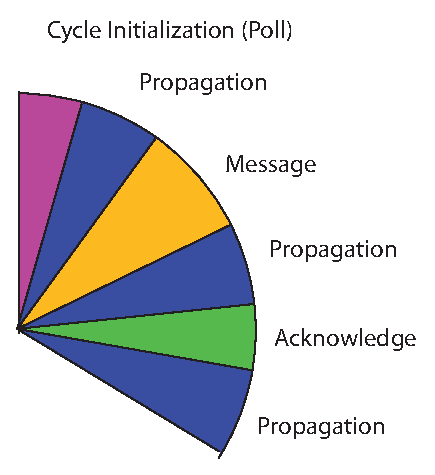
\includegraphics[width=0.2\textwidth]{slots_polled.eps}\label{fig:slots_polled}}\hfil
	\subfloat[Decentralized TDMA]{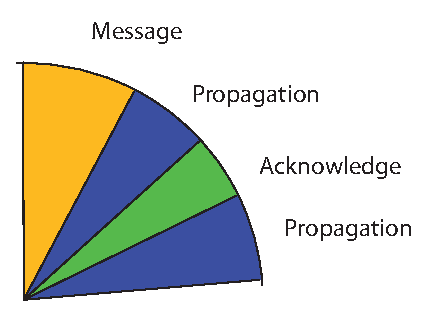
\includegraphics[width=0.2\textwidth]{slots_decentralized.eps}\label{fig:slots_decentralized}}}
\caption{Comparison of the time needed for a single slot for the two types of TDMA supported by pAcommsHandler. Eq. \ref{eq:mac_time} gives the additional length of time required by the Centralized variant.}
\label{fig:slots}
\end{figure}

\begin{figure}
\centering
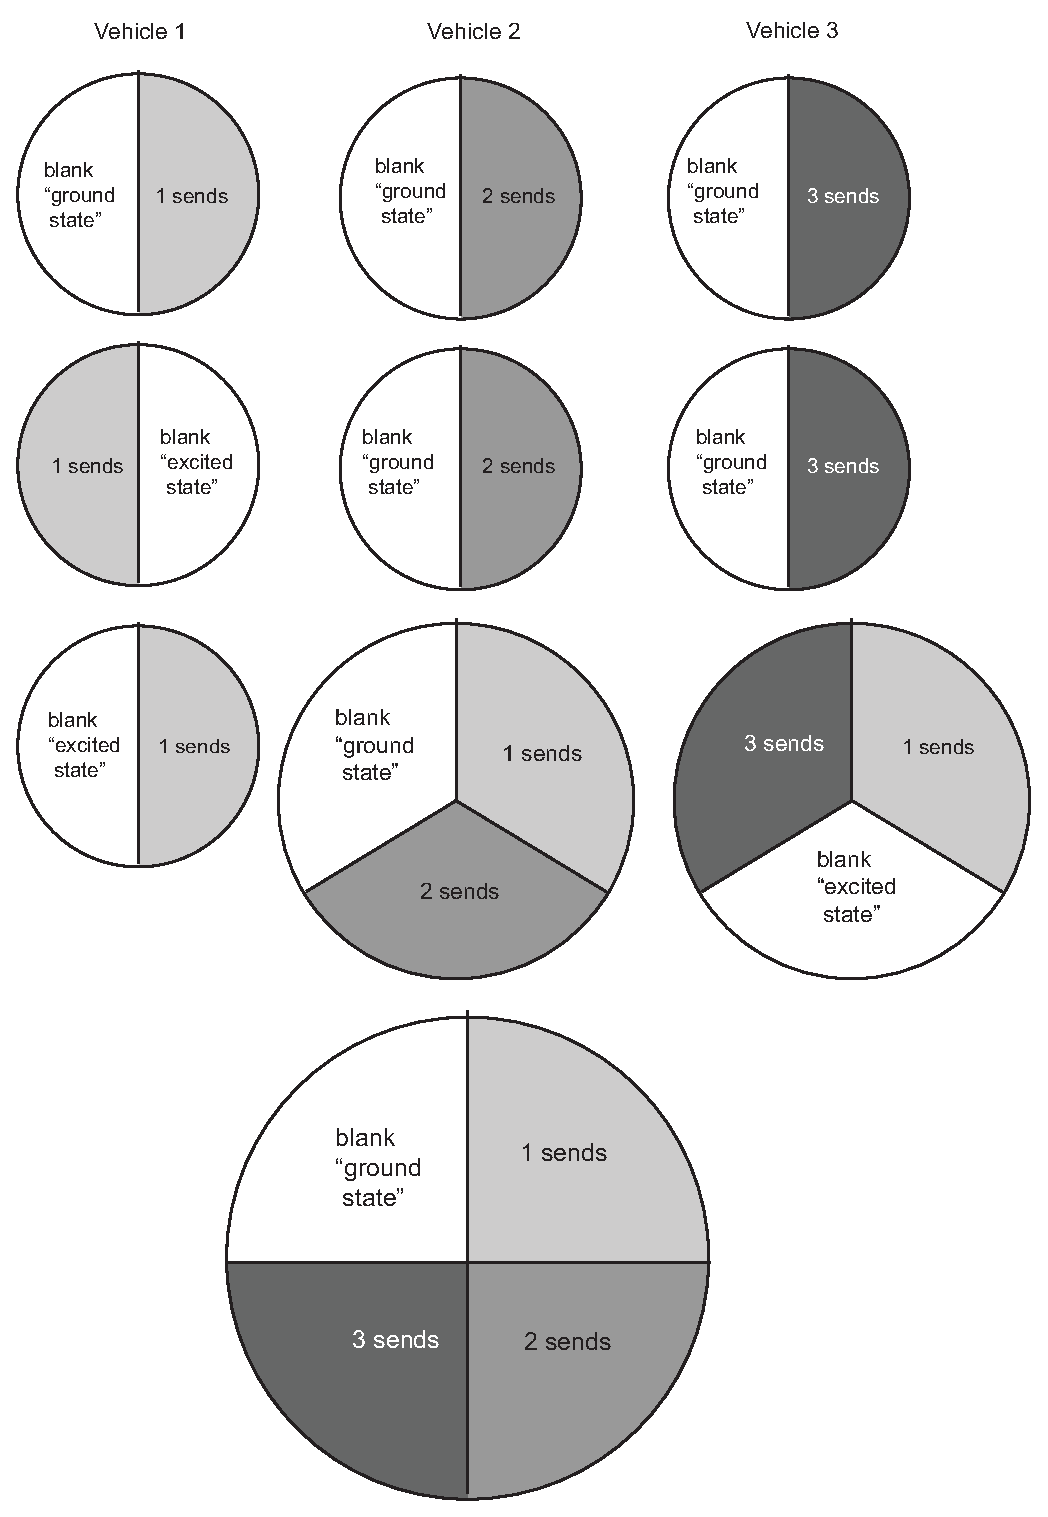
\includegraphics[width=0.5\textwidth]{slots.eps}
\caption{Graphical example of auto discovery for three nodes launched at the same time. Each circle represents the vehicle's cycle at each time step (represented by horizontal rows) based on the vehicle's current knowledge of the world. In the first row, all vehicles only know of themselves and put the blank slot in the last slot; thus, all communications collide and no discoveries are made. In the second row, vehicle 1's blank is moved (by pseudo-chance) to the penultimate (first) slot, so vehicles 2 and 3 discover 1. Then, in the third row vehicles 2 and 3 are discovered by the others because vehicle 3 moves its blank slot. By the fourth row all vehicles have discovered the others and continue to transmit without collision following the cycle diagrammed on this row.} 
\label{fig:decentralized_cycles}
\end{figure}

\subsubsection{Decentralized TDMA with passive auto-discovery}

Decentralized TDMA removes the cycle initialization packet and thus reduces the length of each slot and the chance of errors. However, it introduces the constraint of synchronized clocks\footnote{the accuracy of the clock synchronization can be  low relative to other timing needs such as bi-static sonar. Generally, accuracy better than 0.1 seconds is acceptable; higher inaccuracies can be handled by increasing the guard time on both sides of each slot.} for all nodes, which can be somewhat tricky to maintain underwater.

Decentralized TDMA gives each vehicle a single slot in which it transmits. Each vehicle initiates its own transmission at the start of its slot. Collisions are avoided by each vehicle following the same rules about slot placement within the time window (based on the time of day). All slots are ordered by ascending acoustic MAC address (or ``modem identification number''), which is an unsigned integer unique for each network.

During the runtime of the network, it is often desirable to add or remove nodes. Since the MAC is spread throughout the nodes, there is no easy way to change the cycle during runtime. \textit{libamac} supports passive auto-discovery (and subsequent expiration) of nodes to provide a solution to this problem. This auto-discovery is passive because it requires no control messaging beyond the normal communications between nodes.

Vehicles are discovered by shifting a blank slot in each cycle based on their knowledge of the world and the time of day. If a new vehicle is heard from during the blank, it is added to the listening vehicle's knowledge of the world and hence their cycle. In the simplified situation (which is really a worst case scenario) discovery is defined by a single vehicle transmitting during a cycle and all the others silent (the current slot is not equal to each vehicle's acoustic MAC address).

\begin{table}
\centering
\begin{tabular}{|c|c|c|c|}
\hline time & vehicle 1 & vehicle 2 & result \\ 
\hline 0   & send       & send  & collision \\ 
\hline 15  & blank      & blank & nothing \\ 
\hline 30  & blank      & send  & success: 1 discovers 2 \\ 
\hline 45  & cycle wait & blank & nothing \\ 
\hline 60  & cycle wait & send  & success \\ 
\hline 75  & cycle wait & blank & nothing \\ 
\hline 90  & send       & blank & success: 2 discovers 1 \\ 
\hline 105 & listen for 2 & cycle wait & nothing \\ 
\hline 120 & blank & cycle wait & nothing \\ 
\hline 135 & send & listen for 1 & success \\ 
\hline 150 & listen for 2 & send & success \\ 
\hline 165 & blank & blank & nothing \\ 
\hline 180 & send & listen for 1 & success \\ 
\hline 195 & blank & blank & nothing \\ 
\hline 210 & listen for 2 & send & success \\ 
\hline 
\end{tabular} 
\caption{Example initialization for the Decentralized TDMA with autodiscovery. By 135 seconds, both vehicles have discovered each other and are synchronized. Thus, no more collisions will occur. This scenario assumes that both vehicles always have some data to send during their slot.}
\end{table}

\subsection{Simple complete example MOOS files}

\subsubsection{Example 1: Basic CCL (goby/share/cfg/MOOS/basic\_ccl)}\label{sec:moos_example_1}
This example sends the bytes !0x020304! from node 1 (!mm1!) to node 2 (!mm2!). It shows use of all the parts of pAcommsHandler except the DCCL encoding / decoding unit. I use !iModemSim! here to simulate the WHOI Micro-Modem. This process is available in moos-ivp-local (\url{http://oceanai.mit.edu/moos-ivp/pmwiki/pmwiki.php?n=Support.Milocal}). You can also easily substitute real modems by removing iModemSim references and changing the !serial_port!.

\paragraph{MOOS file for Node 1: goby/share/cfg/MOOS/basic\_ccl/mm1.moos}
\boxedverbatiminput{"@RELATIVE_CMAKE_SOURCE_DIR@/share/cfg/MOOS/basic_ccl/mm1.moos"}
\resetbvlinenumber

\paragraph{MOOS file for Node 2: goby/share/cfg/MOOS/basic\_ccl/mm2.moos}
\boxedverbatiminput{"@RELATIVE_CMAKE_SOURCE_DIR@/share/cfg/MOOS/basic_ccl/mm2.moos"}
\resetbvlinenumber

\subsubsection{Example 2: DCCL and CCL (goby/share/cfg/MOOS/ccl\_and\_dccl)}
This example sends the DCCL ``Simple Status'' messsage from node 1 (!mm1!) to node 2 (!mm2!). !mm2! sends the REMUS CCL State message to !mm1!. It thus uses all the components of pAcommsHandler. As in the previous example, you can use real modems by removing iModemSim and changing the !serial_port! to the proper real serial port.

\paragraph{MOOS file for Node 1: goby/share/cfg/MOOS/ccl\_and\_dccl/mm1.moos}
\boxedverbatiminput{"@RELATIVE_CMAKE_SOURCE_DIR@/share/cfg/MOOS/ccl_and_dccl/mm1.moos"}
\resetbvlinenumber

\paragraph{MOOS file for Node 2: goby/share/cfg/MOOS/ccl\_and\_dccl/mm2.moos}
\boxedverbatiminput{"@RELATIVE_CMAKE_SOURCE_DIR@/share/cfg/MOOS/ccl_and_dccl/mm2.moos"}
\resetbvlinenumber

\paragraph{XML definition of Simple Status: goby/xml/simple\_status.xml}
\boxedverbatiminput{"@RELATIVE_CMAKE_SOURCE_DIR@/share/xml/simple_status.xml"}
\resetbvlinenumber

\paragraph{Modem Lookup Table: goby/share/cfg/MOOS/ccl\_and\_dccl/modemidlookup.txt}
\boxedverbatiminput{"@RELATIVE_CMAKE_SOURCE_DIR@/share/cfg/MOOS/ccl_and_dccl/modemidlookup.txt"}
\resetbvlinenumber

\section{iCommander}\label{sec:icommander} 

\textit{Deprecated. Use goby\_liaison as a replacement.}

\section{pREMUSCodec}

\textit{Deprecated. (**FILL IN DETAILS FOR REPLACEMENT**)}

\DeleteShortVerb{\!}
